\documentclass[10pt]{article}
\usepackage{setspace}
\onehalfspacing
\usepackage[outputdir=build,newfloat]{minted}
\usepackage{algpseudocode}
\usepackage{algorithm}
\usepackage[margin=1.2in]{geometry}
\usepackage{amsmath,amsthm}
\usepackage{mathtools}
\usepackage{enumitem}
\usepackage[colorlinks=true]{hyperref}
\usepackage[capitalize,nameinlink]{cleveref}
\usepackage{amssymb}
\setlist[enumerate]{font=\bfseries}
\theoremstyle{definition}
\newtheorem{question}{Question}
\theoremstyle{remark}
\newtheorem*{solution}{Solution}
\DeclarePairedDelimiter\abs{\lvert}{\rvert}
\DeclarePairedDelimiter\norm{\lVert}{\rVert}
\DeclarePairedDelimiter\vecnorm{\lVert}{\rVert}
\DeclarePairedDelimiter\ip{\langle}{\rangle}
\DeclarePairedDelimiter{\floor}{\lfloor}{\rfloor}
\DeclarePairedDelimiter{\ceil}{\lceil}{\rceil}

\DeclareMathOperator{\diag}{diag}
\DeclareMathOperator{\cond}{cond}
\DeclareMathOperator{\Span}{Span}
\DeclareMathOperator{\arccosh}{arccosh}
\DeclareMathOperator{\sign}{sign}
\DeclareMathOperator{\col}{col}
\DeclareMathOperator{\spectrum}{spectrum}
\DeclareMathOperator*{\trace}{tr}
\DeclareMathOperator*{\argmin}{arg\,min}
\DeclareMathOperator*{\argmax}{arg\,max}

\renewcommand{\leq}{\leqslant}
\renewcommand{\geq}{\geqslant}

\newcommand{\mymarks}[1]{(\textbf{#1 marks})}
\newcommand{\mymark}{(\textbf{1 mark})~}
\newcommand{\mybonus}[1]{(\textbf{Bonus +#1})~}
\renewcommand{\d}{\mathrm d}
\renewcommand{\i}{\mathrm i}
\renewcommand{\t}{T}
\newcommand{\e}{\mathrm e}
\newcommand{\D}{\mathrm D}
\newcommand{\real}{\mathbf R}
\newcommand{\poly}{\mathbf P}
\newcommand{\bigo}{\mathcal O}
\newcommand{\complex}{\mathbf C}
\newcommand{\nat}{\mathbf N}
\newcommand{\integer}{\mathbf Z}
\newcommand{\floating}{\mathbf F}
\newcommand{\madd}{\mathbin{\widehat +}}
\newcommand{\mdiv}{\mathbin{\widehat /}}
\newcommand{\mtimes}{\mathbin{\widehat *}}
\newcommand{\msub}{\mathbin{\widehat -}}
\newcommand{\vect}[1]{\mathbf{\boldsymbol{#1}}}
\newcommand{\mat}{\mathsf}
\newcommand{\placeholder}{\mathord{\color{black!33}\bullet}}%
\newcommand{\moreinfo}{\texorpdfstring{{\normalfont \color{lightred}$^{\text{\faSearchPlus}}$}}{}}
\newcommand{\laplacian}{\triangle}
\newcommand{\expect}{\mathbf E}
\newcommand{\var}{\mathbf V}
\newcommand{\proba}{\mathbf P}
\newcommand{\julia}[1]{\mintinline{julia}{#1}}

% \usepackage{tikz-cd}
% \usetikzlibrary{graphs,graphdrawing}
% \usetikzlibrary{backgrounds}

\theoremstyle{plain}% default
\newtheorem{theorem}{Theorem}
\newtheorem{proposition}[theorem]{Proposition}
\crefname{figure}{Figure}{Figures}

\begin{document}

\title{Numerical Analysis: Final Exam \\
\small{(\textbf{50 marks}, only the 4 best questions count)}}
\author{Urbain Vaes}
\date{December 2024}
\maketitle

\section*{Academic integrity pledge}
\noindent $\square$ \textcolor{blue}{I certify that I will not give or receive any unauthorized help on this exam,
and that all work will be my own. (Tick $\checkmark$ or copy the sentence on your answer sheet)}.


\newpage
\begin{question}
    [Floating point arithmetic, \textbf{10 marks}]
    $~$
    \begin{enumerate}
        \item
            \textbf{(T/F)}
            Let $(\placeholder)_2$ denote base 2 representation.
            It holds that
            \[
                3 \times (0.0101)_2 = (0.1111)_2.
            \]

        \item
            \textbf{(T/F)}
            Does the following equality holds? Explain your reasoning.
            \[
                (0.\overline{011})_2 = \frac{3}{4}.
            \]
             \vspace{1.7cm}

        \item
            \textbf{(T/F)}
            In Julia, \julia{Float64(x) == Float32(x)} is \julia{true} if \julia{x} is a rational number.

        \item
            \textbf{(T/F)}
            The value of the machine epsilon is the same for the double precision format is the same in Julia and Python.

        \item
            \textbf{(T/F)}
            The spacing (in absolute value) between successive double-precision (\julia{Float64}) floating point numbers is equal to the machine epsilon.

        \item
            \textbf{(T/F)}
            All the natural numbers can be represented exactly in the double precision floating point format~\julia{Float64}.

        \item
            \textbf{(T/F)}
            Machine addition in the \julia{Float64} format is associative but not commutative.

        \item
            \textbf{(T/F)}
            In Julia, let \julia{f(x) = (x == x/100.0) ? x : f(x/100.0)}.
            Then \julia{f(a)} returns~\julia{0.0} for all finite number \julia{a} representable in the \julia{Float64} format.

        \item
             In Julia \julia{exp(eps()) == 1 + eps()} evaluates to \julia{true}.
             Explain briefly why.
             \vspace{1.7cm}

        \item
             In Julia \julia{sqrt(1 + eps()) == 1 + eps()} evaluates to \julia{false}.
             Explain briefly why.
             \vspace{1.7cm}
    \end{enumerate}
\end{question}

\newpage
\begin{question}
    [Interpolation, \textbf{10 marks}]
    $~$
    \begin{enumerate}
        \item
            \textbf{(T/F)}
            The only polynomial~$p$ of degree at most 3 such that $p(-1) = p(0) = p(1) = 1$ is the
            constant polynomial~$p(x) = 1$.

        \item
            \textbf{(T/F)}
            In polynomial interpolation, using Chebyshev nodes can help reduce the interpolation error compared to using equidistant nodes.

        \item
            \textbf{(2 marks)}
            Let $S(n) = \sum_{i=1}^{n} i$.
            Given that $S(n)$ is a quadratic polynomial,
            calculate the expression of~$S(n)$ by interpolation.
            Include the details of your calculation.
            \vspace{2.5cm}

        \item
            \textbf{(T/F)}
            Given $x_0 < x_1 < x_2$
            and $y_0, y_1, y_2 \in \mathbb R$,
            the unique polynomial passing through these data points is given by
            \begin{align*}
                p(x) &=
                \frac{(x - x_1) (x-x_2)}{(x_0 - x_1) (x_0 - x_2)} y_0
                + \frac{(x - x_0) (x-x_2) }{(x_1 - x_0) (x_1 - x_2)} y_1
                + \frac{(x - x_0) (x-x_1)}{(x_2 - x_0) (x_2 - x_1)} y_2.
            \end{align*}

        \item
            \textbf{(T/F)}
            Let $f(x) = \exp(5x)$,
            and for any $n \in \mathbb N$,
            let $f_n \in \mathcal P_n$ denote the polynomial interpolating~$f$ at~$n+1$ equidistant points $-1 = x_0 < x_1 < \dotsc < x_n = 1$.
            Then
            \[
                \lim_{n \to \infty} \left( \max_{-1 \leqslant x \leqslant 1} \bigl\lvert f(x) - f_n(x) \bigr\rvert \right) = 0.
            \]

        \item
            \textbf{(2 marks)}
            Given $x_0 < \dotsc < x_n$
            and $y_0, \dotsc, y_n \in \mathbb R$,
            prove that the constant polynomial $p$ that minimizes 
            the expression $\sum_{i=0}^{n} |y_i - p(x_i)|^2$ is given by
            \[
                p(x) = \frac{1}{n+1} \sum_{i=0}^{n} y_i.
            \]
            \vspace{1.0cm}

        \item
            \textbf{(2 marks)}
            We wish to find $a, b, c$ such that the function $f(x) := a \cos(x) + b \sin(x) + c$ 
            interpolates the data points $(0, 0), (1, 1), (2, 2)$.
            Complete on paper the following code for calculating $a, b, c$.
            \begin{minted}{julia}
   x = [0.0, 1.0, 2.0]
   y = [0.0, 1.0, 2.0]
   # Your code below
            \end{minted}
    \end{enumerate}
\end{question}

\newpage
\begin{question}
    [Integration, \textbf{10 marks}]
    $~$
    \begin{enumerate}
        \item
            \textbf{(T/F)}
            The degree of precision of the following quadrature rule is 1:
            \[
                \int_{-1}^{1} f(x) \, \d x
                \approx 2 f(0).
            \]

        \item
            \textbf{(T/F)}
            The closed Newton--Cotes rule with $n$ points is exact for all linear polynomials.

        \item
            \textbf{(T/F)}
            The degree of precision of the following quadrature rule is 5:
            \[
                \int_{-1}^1 f(x) \, \d x \approx 2f(0) + \frac{2}{3} f''(0) + \frac{2}{5} f^{(4)}(0).
            \]

        \item
            \textbf{(T/F)}
            Suppose that $f \in C^{\infty}[a, b]$ and let $I_n[f]$ denote the approximate integral of $f$ using the composite trapezium rule
            with~$n$ integration points.
            Then it holds that
            \[
                \lim_{n \to \infty} \Bigl\lvert I[f] - I_n[f] \Bigr\rvert = 0, \qquad I[f] := \int_{a}^{b} f(x) \, \d x.
            \]

        \item
            \textbf{(T/F)}
            Suppose that $f \in C^{\infty}[a, b]$ and let $I_n[f]$ denote the approximate integral of $f$ using the composite trapezium rule
            with~$n$ integration points.
            Then it holds that
            \[
                \lim_{n \to \infty} n^2 \Bigl\lvert I[f] - I_n[f] \Bigr\rvert = 0.
            \]

        \item
            \textbf{(2 marks)}
            Calculate weights $w_1,w_2$ so that the degree of precision of the following rule is~$1$:
            \[
                \int_{-1}^1 f(x) \, \d x = w_1 f(0) + w_2 f(1).
            \]

        \item
            \textbf{(2 marks)}
            Implement the composite trapezium rule with $n$ points:
            \begin{minted}{julia}
    function I_approx(a, b, n)
        x = LinRange(a, b, n)




            \end{minted}

        \item
            \textbf{(1 mark)}
            The following code implements the midpoint rule with $n$ points, but there is an error.
            Spot and correct the error.
            \begin{minted}{julia}
    function I_approx(n)
        x = LinRange(a, b, n)
        h = (b - a) / n
        return h * sum(f, x .+ h/2)
    end
            \end{minted}
    \end{enumerate}
\end{question}


\newpage
\begin{question}
    [Iterative method for linear systems, \textbf{10 marks}]
    Assume that $\mat A \in \real^{n \times n}$ is a \emph{symmetric positive definite} matrix and that $\vect b \in \real^n$.
    We wish to solve the linear system
    \begin{equation}
        \label{eq:linear_system}
        \mat A \vect x = \vect b.
    \end{equation}
    To this end we consider an iterative method where each iteration is of the form
    \begin{equation}
        \label{eq:iterative_scheme}
        \mat M \vect x_{k+1} = \mat N \vect x_k + \vect b.
    \end{equation}
    Here $\mat A = \mat M - \mat N$ is a splitting of~$\mat A$ such that $\mat M$ is nonsingular,
    and $\vect x_k \in \real^n$ denotes the $k$-th iterate of the numerical scheme.

    \begin{enumerate}
        \itemsep0pt
        \item
            \mymarks{3}
            Let $\vect e_k := \vect x_k - \vect x_*$,
            where $\vect x_*$ is the exact solution to~\eqref{eq:linear_system}.
            Prove that
            \[
                \forall k \in \nat, \qquad
                \vect e_{k+1} = \mat M^{-1} \mat N \vect e_k.
            \]

        \item
            \mymarks{2}
            We denote by $\norm{\placeholder}_{\mat A}$ the vector norm
            \begin{equation}
                \norm{\vect x}_{\mat A} := \sqrt{\vect x^\t \mat A \vect x},
            \end{equation}
            and we use the same notation for the induced matrix norm.
            Prove that
            \begin{equation}
                \label{eq:inequality_interpolation}
                \forall k \in \nat, \qquad
                \norm{\vect e_k}_{\mat A} \leq L^k \norm{\vect e_0}_{\mat A},
                \qquad L := \norm{\mat M^{-1} \mat N}_{\mat A}.
            \end{equation}

        \item
            \mymark
            Is the condition~$\norm{\mat M^{-1} \mat N}_{\mat A} < 1$ sufficient to ensure convergence for all~$\vect x_0$?

        \item
            *\mymarks{3}
            Show that
            \begin{equation}
                \label{eq:norm}
                \norm{\mat M^{-1} \mat N \vect x}_{\mat A}^2
                = \norm{\vect x}_{\mat A}^2 - \vect y^\t (\mat M^\t + \mat N) \vect y,
                \qquad \vect y :=  \mat M^{-1} \mat A \vect x.
            \end{equation}

            \textbf{Hint: } Eliminate~$\mat N$ from both sides of the equation by rewriting~$\mat N = \mat M - \mat A$.
            Then substitute the expression of~$\vect y$ and expand both sides.
            Remember that a scalar quantity transposed is equal to itself.

        \item
            \mymark
            Show that, for the Gauss--Seidel method,
            i.e.\ when $\mat M = \mat L + \mat D$ contains just the lower triangular and diagonal parts of~$\mat A$,
            it holds that
            \begin{equation}
                \label{eq:gauss_seidel}
                \mat M^\t + \mat N = \mat D.
            \end{equation}

        \item
            \mybonus{2}
            Deduce from~\eqref{eq:norm} and~\eqref{eq:gauss_seidel} that,
            for the Gauss--Seidel method,
            \[
                \norm{\mat M^{-1} \mat N}_{\mat A} < 1.
            \]
    \end{enumerate}
\end{question}

\newpage
\begin{question}
    [Nonlinear equations, \textbf{10 marks}]
    We consider the following iterative method for calculating~$\sqrt[3]{2}$:
    \begin{equation}
        \label{eq:iteration}
        x_{k+1} = F(x_k) :=  \omega x_k + (1 - \omega) \frac{2}{x_k^2},
    \end{equation}
    with $\omega \in (0, 1)$ a fixed parameter.
    \begin{enumerate}
        \item
            \mymark
            Show that $x_* := \sqrt[3]{2}$ is a fixed point of the iteration~\eqref{eq:iteration}.

        \item
            \mymarks{2}
            Write down in pseudocode a computer program based on the iteration~\eqref{eq:iteration} for calculating~$\sqrt[3]{2}$.
            Use an appropriate stopping criterion that does not require to know the value of~$\sqrt[3]{2}$.

        \item
            \mymarks{2}
            Prove that if~$\omega \in \left(\frac{1}{3}, 1\right)$,
            then~$x_*$ is locally exponentially stable.
            You may take for granted~\cref{proposition:local_convergence} at the end of this document.

        \item
            \mymark
            Do you expect faster convergence of~\eqref{eq:iteration} with $\omega = \frac{1}{2}$ or with $\omega = \frac{2}{3}$?

        \item
            \mymarks{2}
            % Write down, in the form
            % \[
            %     x_{k+1} = \dots
            % \]
            Show that, in the particular case where $\omega = \frac{2}{3}$,
            the iterative scheme~\eqref{eq:iteration} coincides with the Newton--Raphson method applied to
            the nonlinear equation
            \begin{equation}
                \label{eq:nonlinear_equation}
                f(x) = 0,
            \end{equation}
            for an appropriate function $f \colon \real \to \real$.
            % Write explicitly the definition of~$f(x)$.

        \item
            \mymarks{2}
            Illustrate graphically a few iterations of the Newton--Raphson method for solving~\eqref{eq:nonlinear_equation} when starting from~$x_0 = 2$.
            You may either create your own figure or write on \cref{fig:nr} at the end of this document.

        \item
            *\mybonus{2}
            Prove~\cref{proposition:local_convergence} in the appendix.
            More precisely, show that the assumptions of the proposition imply that there is $\delta > 0$ and $L < 1$ such that the following local Lipschitz condition is satisfied:
            \begin{equation}
                \label{eq:local_lipschitz}
                \forall x \in [x_* - \delta, x_* + \delta],
                \qquad
                \lvert F(x) - F(x_*) \rvert \leq L \abs{x - x_*}.
            \end{equation}
            For completeness, one should then show that~\eqref{eq:local_lipschitz} is sufficient to guarantee local exponential stability,
            but this is taken for granted here; you do not need to prove this.
    \end{enumerate}
\end{question}

\newpage

\newpage

\newpage
\begin{question}
    [Iterative methods for eigenvalue problems, \textbf{10 marks}]
    Let $\norm{\placeholder}$ denote both the Euclidean norm on vectors and the induced matrix norm.
    Assume that~$\mat A \in \real^{n \times n}$ is symmetric and nonsingular,
    and that all the eigenvalues of~$\mat A$ have different moduli:
    \[
        \lvert \lambda_1 \rvert
        >
        \lvert \lambda_2 \rvert
        >
        \dots
        >
        \lvert \lambda_n \rvert.
    \]

    \begin{enumerate}
        \item
            \mymarks{5}
            Describe with words and pseudocode a simple numerical method for calculating the eigenvalue of $\mat A$ of smallest modulus
            as well as the corresponding eigenvector.

        \item
            \mymarks{2}
            Suppose that we have calculated the smallest eigenvalue in modulus $\lambda_n$,
            as well as the associated normalized eigenvector~$\vect v_n$.
            We let
            \[
                \mat B := \mat A^{-1} - \frac{1}{\lambda_n} \vect v_n \vect v_n^\t.
            \]
            % Write down an expression for the eigenvalues of~$\mat B$ in terms of the eigenvalues of~$\mat A$.
            If we apply the power iteration to this matrix,
            what convergence can we expect?
            Justify your answer.


        \item
            *\mymarks{3}
            The aim of this part is to provide an answer to the following question:
            given an approximate eigenpair $(\widehat {\vect v}, \widehat \lambda)$,
            what is the smallest perturbation~$\mat E$ that we need to apply to $\mat A$ in order to guarantee that
            $(\widehat {\vect v}, \widehat \lambda)$ is an exact eigenpair, i.e.\ that
            \[
                (\mat A + \mat E) \widehat {\vect v} = \widehat \lambda \widehat {\vect v} \,?
            \]
            Assume that $\widehat {\vect v}$ is normalized and
            let $\mathcal E = \Bigl\{\mat E \in \complex^{n \times n}: (\mat A + \mat E) \widehat {\vect v} = \widehat \lambda \widehat {\vect v} \Bigr\}$.
            Prove that
            \begin{equation}
                \label{eq:kahan_parlett_jiang}
                \min_{\mat E \in \mathcal E} \norm{\mat E} = \norm{\vect r}, \qquad \vect r := \mat A \widehat {\vect v} - \widehat \lambda \widehat {\vect v}.
            \end{equation}
            \textbf{Hint:} You may find it useful to proceed as follows:
            \begin{itemize}
                \item
                    Show first that $\mat E \in \mathcal E$ if and only if $\mat E \widehat {\vect v} = - \vect r$.

                \item
                    Deduce from the previous item that
                    \[
                        \forall \mat E \in \mathcal E, \qquad
                        \norm{\mat E} \geq \norm{\vect r}.
                    \]

                \item
                    Find a rank one matrix $\mat E_* \in \mathcal E$ such that
                    \(
                    \norm{\mat E_*} = \norm{\vect r},
                    \)
                    and then conclude.
                    Recall that any rank 1 matrix can be written in the form $\mat E_* = \vect u \vect w^*$,
                    with norm $\norm{\vect u} \norm{\vect w}$.
            \end{itemize}

        \item
            \mybonus{2}
            Suppose that we have calculated~$\lambda_n$ and $\lambda_{n-1}$ together with the associated normalized eigenvectors.
            Propose a method for calculating the third smallest eigenvalue in modulus, i.e.\ $\lambda_{n-2}$.
    \end{enumerate}
\end{question}



\newpage

\section*{Auxiliary results}
\begin{proposition}
    \label{proposition:interpolation_error}
    Assume that~$f\colon [a, b] \to \real$ is a function in $C^{2}([a, b])$ and let $\widehat f$ denote
    the interpolation of~$f$ at two distinct interpolation nodes~$y_1, y_2$.
    Then there exists~$\xi\colon [a, b] \to [a, b]$ such that
    \[
        \forall y \in [a, b], \qquad
        f(y) - \widehat f(y) = \frac{f''\bigl(\xi(y)\bigr)}{2} (y-y_1) (y - y_2).
    \]
\end{proposition}

\begin{proposition}
    \label{proposition:local_convergence}
    Assume that $F\colon (0, \infty) \to (0, \infty)$ is continuously differentiable,
    and suppose that~$x_* \in (0, \infty)$ is a fixed point of the iteration
    \(
        x_{k+1} = F(x_k).
    \)
    If
    \[
        \abs{F'(x_*)} < 1,
    \]
    then the fixed point $x_*$ is locally exponentially stable.
\end{proposition}

\begin{figure}[ht]
    \centering
    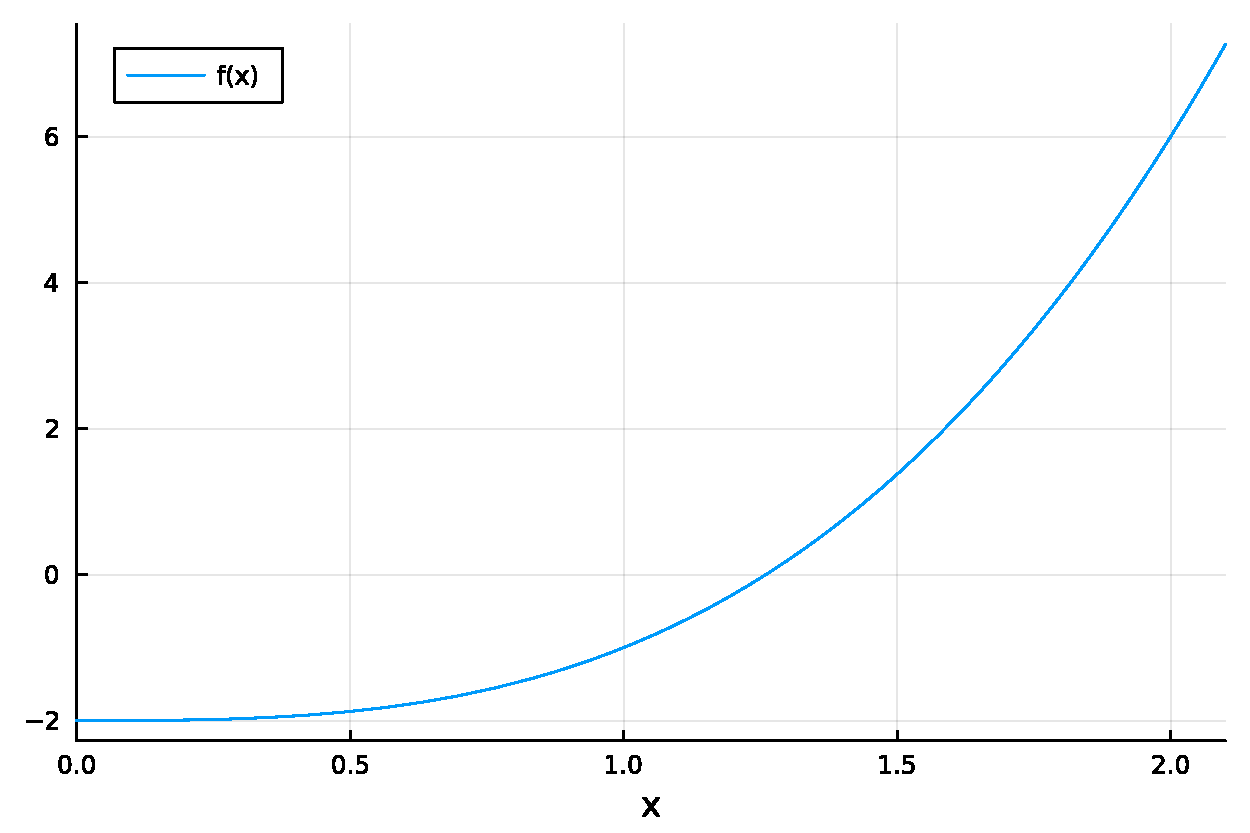
\includegraphics[width=\linewidth]{newton-raphson.pdf}
    \caption{You can use this figure to illustrate the Newton--Raphson method.}%
    \label{fig:nr}
\end{figure}

\end{document}
